\documentclass[11pt]{article}
\usepackage[toc,page]{appendix}
\usepackage{amsmath, amssymb}
\usepackage[utf8]{inputenc}
\usepackage[T1]{fontenc}
\usepackage[style=apa,backend=biber]{biblatex}
%\usepackage{biblatex}
\addbibresource{references.bib}
\usepackage{graphicx}
\usepackage{tikz}
\usetikzlibrary{automata,positioning,shapes.geometric, arrows.meta, fit, backgrounds, calc, chains}
\graphicspath{./images/Easy_Pictures/SMR_MULT_Repackaging}%\usepackage{kpfonts}
\usepackage{float}
\usepackage[margin=1in]{geometry}
\usepackage{cancel}
\usepackage{epsfig}
\usepackage{tikz-3dplot}
\usepackage{darkmode}
\usepackage{dirtytalk}
\usepackage{longtable,booktabs,array}
\usepackage{calc} % for calculating minipage widths
\usepackage[utf8]{inputenc}
\usepackage[T1]{fontenc}
\usepackage{xcolor}
\usepackage{listings}


\usepackage{etoolbox}
\usepackage{hyperref}
\hypersetup{
 colorlinks=true,
 linkcolor=blue,
 filecolor=magenta, 
 urlcolor=cyan,
 pdftitle={Hermeneutic Calculator},
 citecolor=blue,
 }


\urlstyle{same}

\lstdefinestyle{htmlStyle}{
 language=HTML,
 basicstyle=\ttfamily\small,
 keywordstyle=\color{blue}\bfseries,
 commentstyle=\color{gray}\itshape,
 stringstyle=\color{red},
 breaklines=true,
 frame=single,
 numbers=left,
 numberstyle=\tiny\color{gray},
 columns=fullflexible,
}
\lstdefinelanguage{HTML}{
 keywords={<!DOCTYPE, html, head, title, body, h1, h2, h3, p, div, span, a, img, ul, li, table, tr, td, th, style, link, script},
 sensitive=true,
 comment=[l]{//},
 morecomment=[s]{/*}{*/},
 morestring=[b]',
 morestring=[b]"
}
\lstset{style=htmlstyle, language=html}
% Updated to explicitly pass the language option
%\lstinputlisting[style=htmlstyle, language=html]{./html/example.html}
%\usepackage{tocloft}

% Optional: define some custom colors
\definecolor{sliceRed}{RGB}{225,224,91} % matching "varyellow" from your code
\definecolor{linkYellow}{RGB}{255,215,0} % a golden yellow
\tdplotsetmaincoords{70}{110}

\title{Subtraction Strategies: Rounding and Adjusting}
\author{Compiled by Theodore M. Savich}


\begin{document}
\maketitle
\subsection*{Rounding and Adjusting}


\subsection*{Transcript}
Video from \textcite{Carpenter1999}. Strategy descriptions and curation by Amy Hackenberg. 

\begin{itemize}
\item \textbf{Teacher:} Kevin had 84 gumdrops. During the week, he ate 29 gumdrops. How many gumdrops does he have left?
\item \textbf{Kevin:} 55. 
\item \textbf{Teacher:} How'd you get 55? 
\item \textbf{Kevin:} I knew if I had 80 gumdrops and I ate 20, I knew I would have 60 gumdrops. But I had to add 4 more because it was 84 minus 20, so that would be 64. And I took away 4 more, and that would be 60. But I had to take away 5 more and that would be 55. 
\end{itemize}

\subsection*{Picture}
\begin{center}
    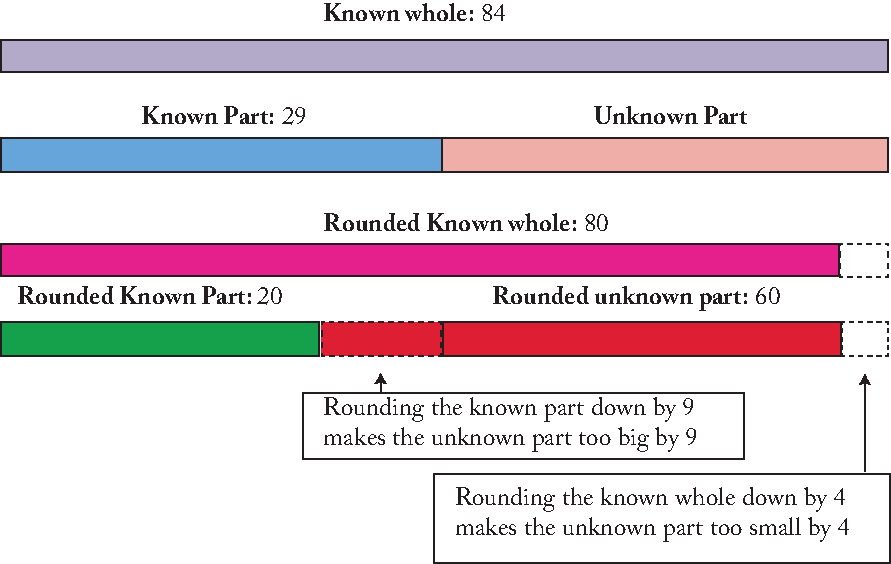
\includegraphics[width=.8\textwidth]{./images/Easy_Pictures/SAR_SUB_ROUNDING_PICTURES/PDF/SAR_SUB_Rounding.pdf}
\end{center}
\subsection*{Notation}
\textbf{Rounding}


\begin{eqnarray}
84-29 = \Box\\
84-4 = 80\\
29-9 = 20\\
80-20 = 60
\end{eqnarray}


\textbf{Adjusting}

\begin{eqnarray}
60+4 = 64\\
64-4 = 60\\
60-5 = 55
\end{eqnarray}


\subsection*{Explaining the Adjusting}
\begin{itemize}
    \item Kevin knew that if he had 80 gumdrops and ate 20, he would have 60 gumdrops left.
    \item Rounding the known whole down by 4 makes the unknown part too small by 4. 
    \item So, adjust the difference by adding 4 gumdrops back to get 64.
    \item Rounding the known part down by 9 makes the unknown part too big by 9
    \item So, adjust the difference by subtracting 9. Kevin does this by chunking back by 4 (to get 60) and then by 5 (to get 55).
\end{itemize}

\subsubsection*{Description of Strategy}
Change either the known part or the known whole to a ``good'' number—usually the nearest base—to make the subtraction easier. Then subtract and adjust your answer. This extra adjusting step can be a bit trickier than rounding when you add!
\begin{itemize}
\item If you round the known whole up, you pretend you had more than you really did, so the unknown part seems too big.
\item If you round the known whole down, you act like you had less, and you'll need to add back what you subtracted at the end. 
\item Similarly, if you round the known part down, you're not subtracting enough and must add back in. 
\item If you round the known part up, you subtract too much and need to add some back to fix it.
\end{itemize}

 







\subsubsection*{Corrected Automaton (Register Machine Model)}

We define a Register Machine that models Kevin's double-rounding strategy, including the iterative chunking used during the final adjustment.

**M = (Q, V, \delta, q_0, F)**

\begin{itemize}
    \item \textbf{States (Q):} {$q_{start}, q_{round\_M}, q_{round\_S}, q_{subtract}, q_{adjust\_M}, q_{init\_adjust\_S}, q_{loop\_adjust\_S}, q_{accept}$}
    \item \textbf{Registers (V):} M\_rounded, S\_rounded, K\_M (adjustment for M), K\_S (adjustment for S), TempResult, K\_S\_Remaining, Chunk.
\end{itemize}

**Key Transitions (\delta):**

\begin{longtable}{|l|l|l|l|l|}
\hline
\textbf{Current State} & \textbf{Condition} & \textbf{Next State} & \textbf{Action} & \textbf{Interpretation} \\
\hline
\endhead
$q_{round\_M}$ & - & $q_{round\_S}$ & M\_r = RoundDown(M); K\_M = M-M\_r & Round M down. Store K\_M. \\
\hline
$q_{round\_S}$ & - & $q_{subtract}$ & S\_r = RoundDown(S); K\_S = S-S\_r & Round S down. Store K\_S. \\
\hline
$q_{subtract}$ & - & $q_{adjust\_M}$ & TempResult = M\_r - S\_r & Calculate intermediate result. \\
\hline
$q_{adjust\_M}$ & - & $q_{init\_adjust\_S}$ & TempResult += K\_M & Compensate for M (Add back). \\
\hline
$q_{init\_adjust\_S}$ & - & $q_{loop\_adjust\_S}$ & K\_S\_Remaining = K\_S & Initialize S adjustment (Subtract). \\
\hline
$q_{loop\_adjust\_S}$ & **K\_S\_Rem > 0** & $q_{loop\_adjust\_S}$ & Calculate strategic Chunk (C); TempResult-=C; K\_S\_Rem-=C & Iterative chunking (Inverse RMB). \\
\hline
$q_{loop\_adjust\_S}$ & **K\_S\_Rem == 0** & $q_{accept}$ & Result = TempResult & Finished. \\
\hline
\end{longtable}

\subsubsection*{Python Implementation and Test}

\begin{lstlisting}[language=Python]
import pandas as pd
import math

class SubtractionRoundingKevin:
    """
    A Register Machine model simulating Kevin's double-rounding strategy (e.g., 84-29).
    Rounds both M and S down, calculates intermediate result, and adjusts sequentially,
    incorporating strategic chunking for the final adjustment.
    """
    strategy_name = "Subtraction Rounding (Kevin's Double Round Down)"

    def __init__(self, M, S, Base=10):
        self.M = M
        self.S = S
        self.Base = Base
        self.history = []
        self.state = 'q_start'
        self.Result = 0

        # Registers
        self.M_rounded = 0; self.K_M = 0 # Adjustment for M (Amount rounded down)
        self.S_rounded = 0; self.K_S = 0 # Adjustment for S (Amount rounded down)
        self.TempResult = 0

        # Internal registers for iterative adjustment (Chunking K_S)
        self.K_S_Remaining = 0
        self.Chunk = 0

        if S > M:
            self.state = 'q_error'
            self._record_history(f"Error: Subtrahend ({S}) > Minuend ({M}).")

    def _record_history(self, interpretation, highlight=False):
        record = {
            'State': self.state, 'Interpretation': interpretation,
            'K_M': self.K_M, 'K_S': self.K_S, 'TempResult': self.TempResult,
            'Highlight': highlight
        }
        # Add K_S_Remaining only if it's relevant (during the adjustment loop)
        if self.state.startswith('q_loop_adjust_S') or self.state.startswith('q_init_adjust_S'):
             record['K_S_Rem'] = self.K_S_Remaining

        self.history.append(record)

    def transition(self, next_state):
        self.state = next_state

    def run(self):
        while self.state not in ['q_accept', 'q_error']:
            executor = getattr(self, f"execute_{self.state}", self.execute_error)
            executor()
        return self.Result

    def execute_error(self):
        if self.state != 'q_error':
            self._record_history(f"Error: Entered unknown state {self.state}")
            self.transition('q_error')

    # --- State Execution Methods ---

    def execute_q_start(self):
        self._record_history(f"Inputs: M={self.M}, S={self.S}.", highlight=True)
        self.transition('q_round_M')

    def execute_q_round_M(self):
        """Round M down to the nearest base."""
        # Models the cognitive step of identifying the lower base and the difference.
        self.K_M = self.M % self.Base
        self.M_rounded = self.M - self.K_M
        self._record_history(f"Round M down: {self.M} -> {self.M_rounded}. (K_M = {self.K_M}).")
        self.transition('q_round_S')

    def execute_q_round_S(self):
        """Round S down to the nearest base."""
        self.K_S = self.S % self.Base
        self.S_rounded = self.S - self.K_S
        self._record_history(f"Round S down: {self.S} -> {self.S_rounded}. (K_S = {self.K_S}).")
        self.transition('q_subtract')

    def execute_q_subtract(self):
        """Calculate the intermediate result."""
        self.TempResult = self.M_rounded - self.S_rounded
        self._record_history(f"Intermediate Subtraction: {self.M_rounded} - {self.S_rounded} = {self.TempResult}.", highlight=True)
        self.transition('q_adjust_M')

    def execute_q_adjust_M(self):
        """Adjust for M. M was rounded down (result too small). Add K_M back."""
        prev = self.TempResult
        self.TempResult += self.K_M
        self._record_history(f"Adjust for M (Add K_M): {prev} + {self.K_M} = {self.TempResult}.", highlight=True)
        self.transition('q_init_adjust_S')

    def execute_q_init_adjust_S(self):
        """Initialize adjustment for S. S was rounded down (result too big). Subtract K_S."""
        self.K_S_Remaining = self.K_S
        if self.K_S_Remaining > 0:
            self._record_history(f"Begin Adjust for S (Subtract K_S): Need to subtract {self.K_S_Remaining}.")
            self.transition('q_loop_adjust_S')
        else:
            # If K_S was 0, proceed to the loop to finalize
            self.transition('q_loop_adjust_S')

    def execute_q_loop_adjust_S(self):
        """Iteratively subtract K_S using strategic chunking (as Kevin did)."""
        if self.K_S_Remaining == 0:
            self.Result = self.TempResult
            self._record_history(f"Adjustment for S complete. Final Result = {self.Result}.", highlight=True)
            self.transition('q_accept')
            return

        # Determine the strategic chunk (subtract down to the previous base - Inverse RMB)
        # Models Kevin's move from 64 -> 60 (Chunk=4) before subtracting the rest (5).

        K_to_prev_base = self.TempResult % self.Base

        if K_to_prev_base > 0 and self.K_S_Remaining >= K_to_prev_base:
             # Sufficient remaining to reach the previous base
             self.Chunk = K_to_prev_base
        else:
             # Either already at a base, or insufficient remaining. Subtract what's left.
             self.Chunk = self.K_S_Remaining

        # Apply the chunk
        prev = self.TempResult
        self.TempResult -= self.Chunk
        self.K_S_Remaining -= self.Chunk

        interpretation = f"Chunking Adjustment: {prev} - {self.Chunk} = {self.TempResult}."
        # Add interpretation note if a boundary was reached
        if self.TempResult % self.Base == 0 and self.Chunk > 0 and prev % self.Base != 0:
             interpretation += " (Reached base boundary)."

        self._record_history(interpretation)
        # Loop back to q_loop_adjust_S

    def display_history(self):
        print(f"\n--- {self.strategy_name} History ({self.M} - {self.S}) ---")
        df = pd.DataFrame(self.history)
        # Determine columns to display, handling the optional K_S_Rem
        display_cols = ['State', 'Interpretation', 'K_M', 'K_S', 'TempResult']
        if 'K_S_Rem' in df.columns:
             display_cols.append('K_S_Rem')

        if not df.empty:
            # Fill NaNs for cleaner display where K_S_Rem is not applicable
            df = df[display_cols].fillna('')

        print(df.to_markdown(index=False))

# Test Case: Kevin's example (84 - 29)
M_test = 84
S_test = 29
kevin_strategy = SubtractionRoundingKevin(M=M_test, S=S_test)
result = kevin_strategy.run()
kevin_strategy.display_history()
\end{lstlisting}

\subsubsection*{Execution Trace (84 - 29):}
\begin{verbatim}
--- Subtraction Rounding (Kevin's Double Round Down) History (84 - 29) ---
| State           | Interpretation                                                       |   K_M |   K_S |   TempResult | K_S_Rem   |
|:----------------|:---------------------------------------------------------------------|------:|------:|-------------:|:----------|
| q_start         | Inputs: M=84, S=29.                                                  |     0 |     0 |            0 |           |
| q_round_M       | Round M down: 84 -> 80. (K_M = 4).                                   |     4 |     0 |            0 |           |
| q_round_S       | Round S down: 29 -> 20. (K_S = 9).                                   |     4 |     9 |            0 |           |
| q_subtract      | Intermediate Subtraction: 80 - 20 = 60.                              |     4 |     9 |           60 |           |
| q_adjust_M      | Adjust for M (Add K_M): 60 + 4 = 64.                                 |     4 |     9 |           64 |           |
| q_init_adjust_S | Begin Adjust for S (Subtract K_S): Need to subtract 9.               |     4 |     9 |           64 | 9         |
| q_loop_adjust_S | Chunking Adjustment: 64 - 4 = 60. (Reached base boundary).           |     4 |     9 |           60 | 5         |
| q_loop_adjust_S | Chunking Adjustment: 60 - 5 = 55.                                    |     4 |     9 |           55 | 0         |
| q_loop_adjust_S | Adjustment for S complete. Final Result = 55.                        |     4 |     9 |           55 | 0         |
\end{verbatim}

\end{document}